\begin{figure*}[htbp]
\centering
\begin{subfigure}[t]{0.45\linewidth}
\centering
\textbf{Pick Bellwether Environment}\\[0.5cm]
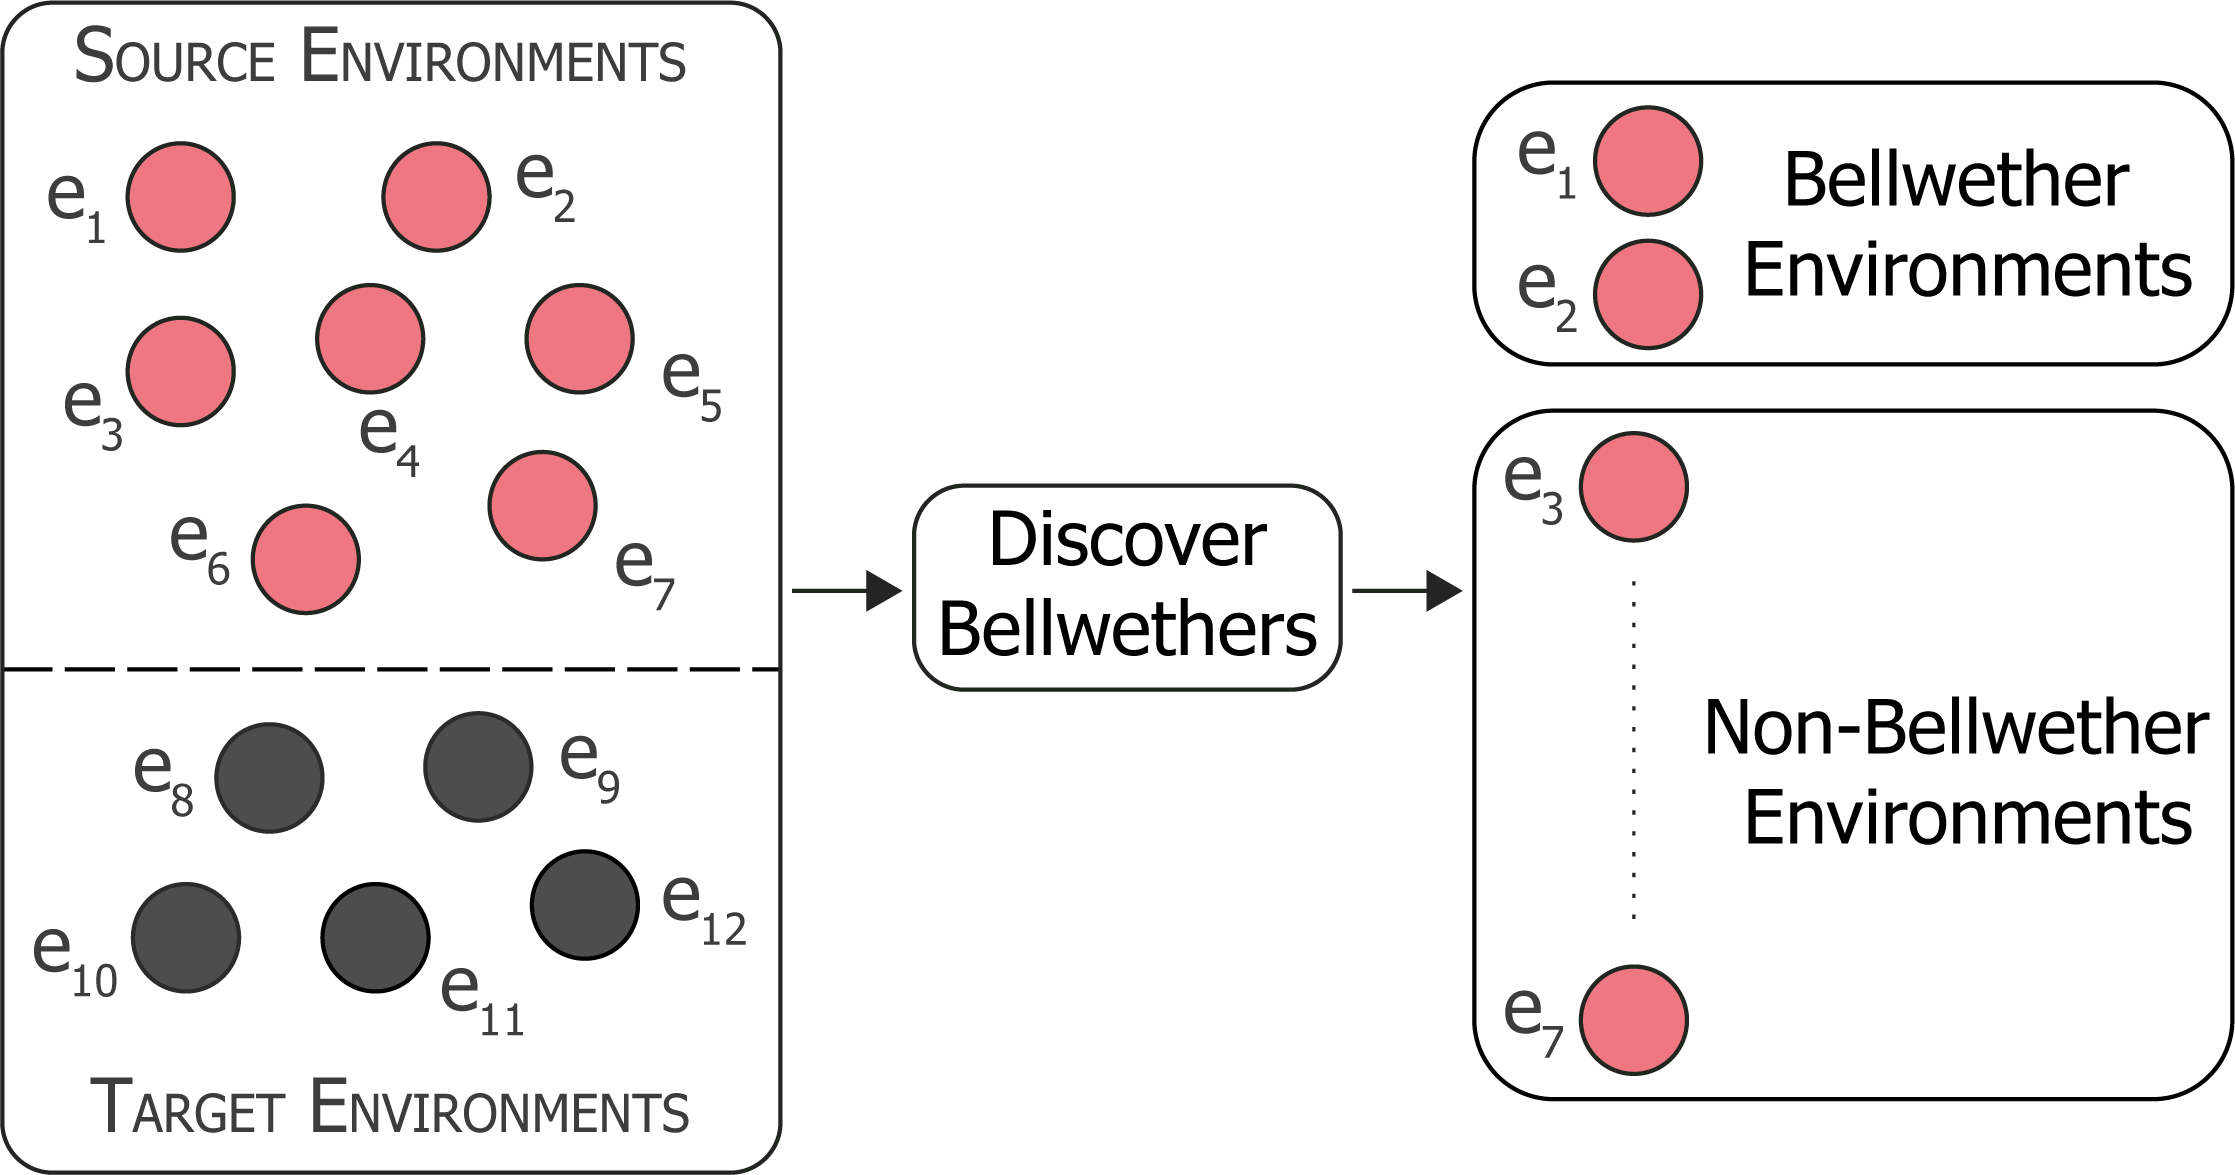
\includegraphics[width=\linewidth]{figures/source_target.png}
\end{subfigure}\hspace{5pt}
\begin{subfigure}[t]{0.5\linewidth}
\hspace{0.4\linewidth}\textbf{Pseudocode}
\small
\begin{lstlisting}[xleftmargin=8.0ex,mathescape,frame=none,numbers=left]
def FindBellwether(sources, step_size, budget, thres, lives): 
  while lives or cost > budget:
    "Sample configurations"
    sampled = list()
    for source in sources:
      sampled += source.sample(step_size)
    "Get cost"
    cost = get_cost(sampled)
    "Evaluate pair-wise performances"
    perf = get_perf(sampled)
    "Remove non-bellwether environments"
    sources = remove_non_bellwethers(sources, perf, thres)
    "Loose life if no sources are removed"
    if prev == len(sources): lives -= 1
    "Return a bellwether"
  return sources[argmin(perf)]
\end{lstlisting}
\end{subfigure}\\[0.4cm]
\begin{subfigure}[t]{0.5\linewidth}
\centering
\textbf{Transfer Learning with Bellwether Environment}\\
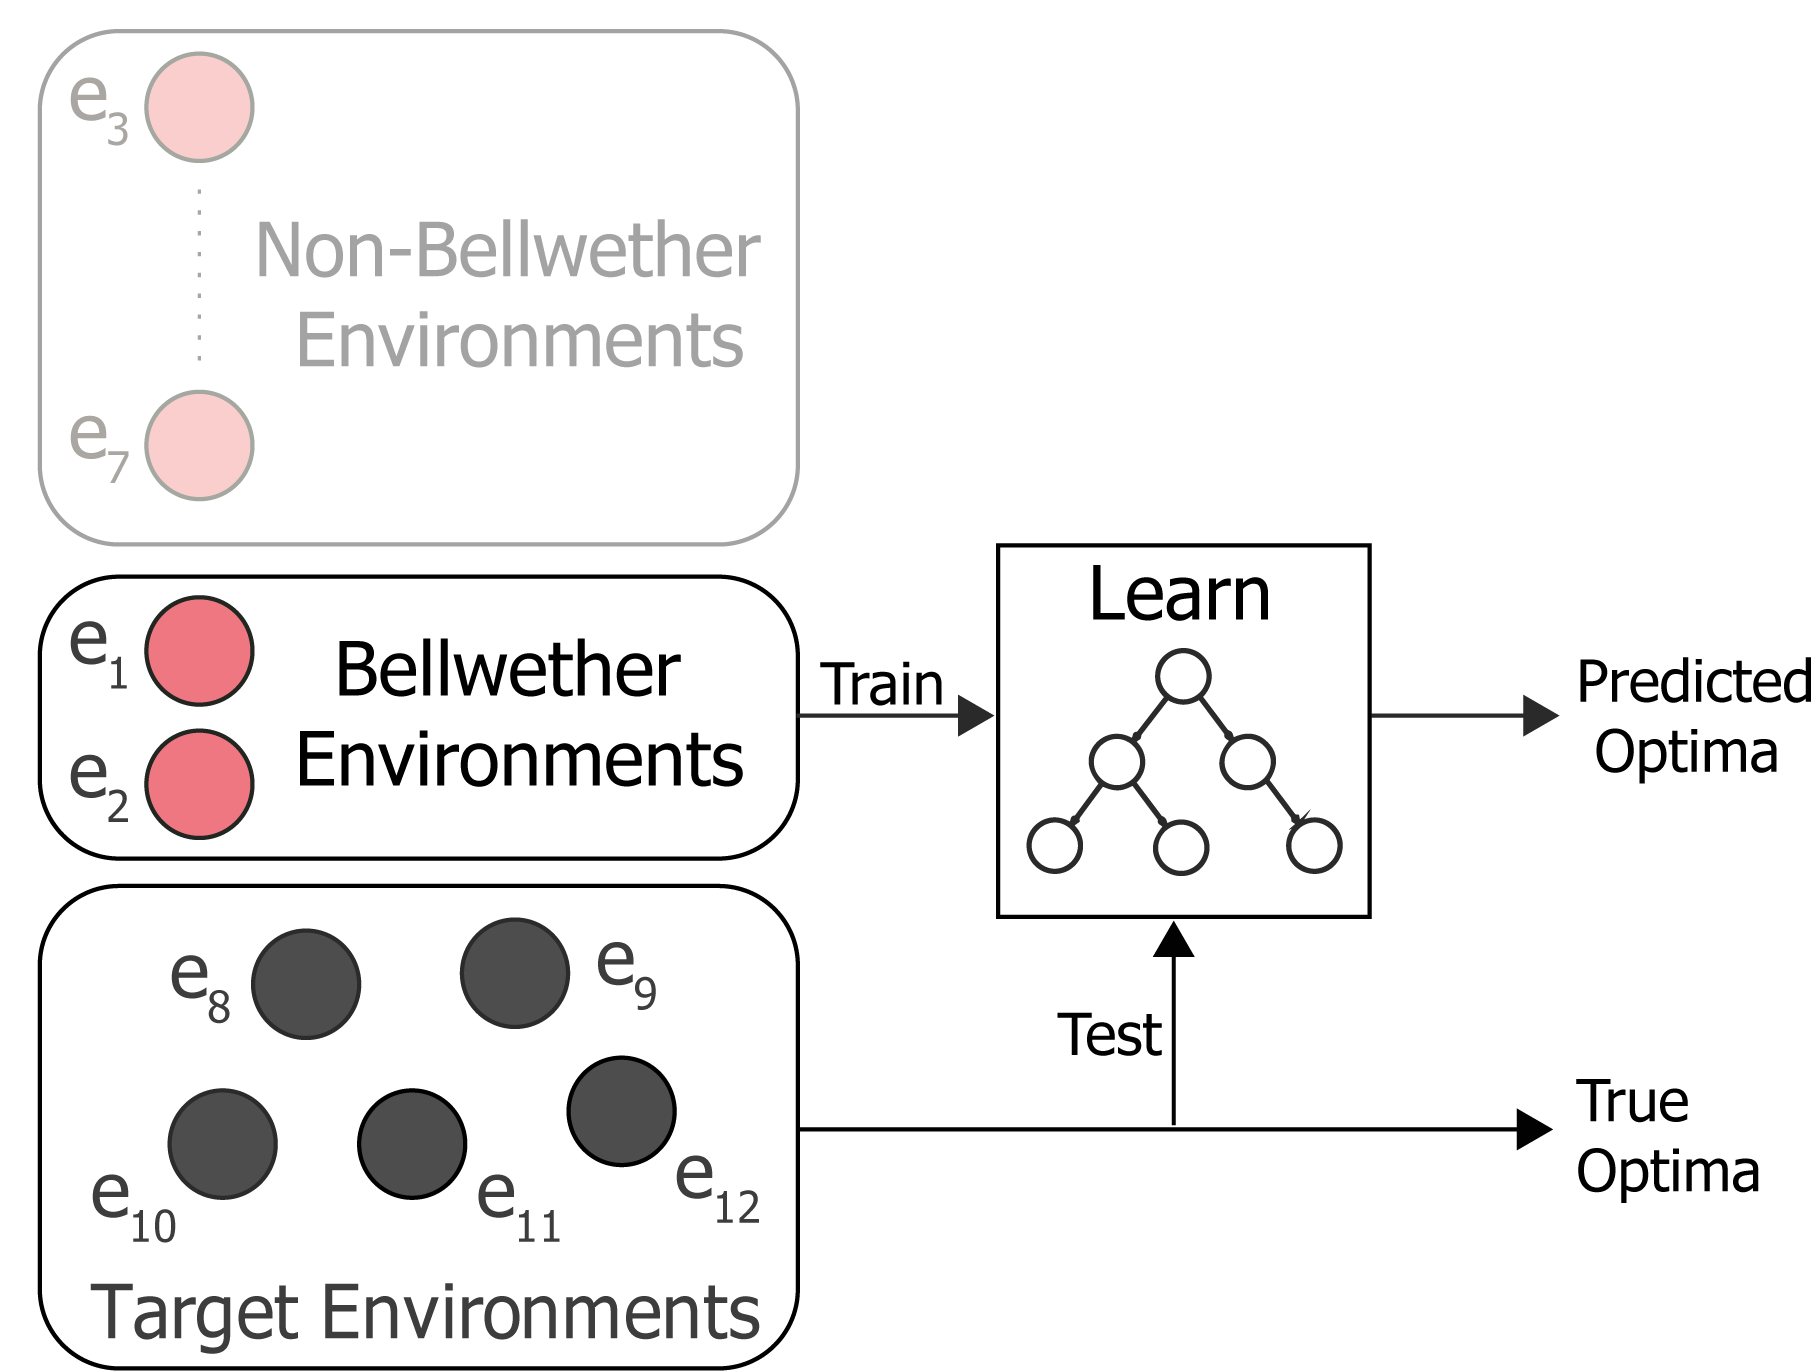
\includegraphics[width=0.85\linewidth]{figures/bellwether-transfer.png}
\end{subfigure}~~%
\begin{subfigure}[t]{0.5\linewidth}
\vspace{0.4cm}
\hspace{0.4\linewidth}\textbf{Pseudocode}\\[-0.3cm]
\small
\begin{lstlisting}[xleftmargin=5.0ex,mathescape,frame=none,numbers=left]
def BEETLE(sources, target, budget): 
    "Find the bellwether environment"
    bellwether = FindBellwether(sources, step_size, budget, thres, lives)
    "Sample the bellwether source to fit budget"
    b_some = bellwether.sample(budget)
    "Train a prediction model with the bellwether"
    prediction_model = regTree.train(b_some)
    predicted = prediction_model.test(target.indep)
    return target[argmin(predicted)]
\end{lstlisting}
\end{subfigure}	
\caption{{\small This figure demonstrates the two key aspects of our proposed approach for transfer learning (a)~how to pick the bellwether environment; (b)~How to construct a  transfer learner with the bellwether environment. A visual intuition of each of the two methods is presented on the left and the corresponding pseudocode are presented on the right.}}
\label{fig:approach}
\end{figure*}